% Figure and table environments with captions: the float files of the paper, in order of appearance.

% Fig. 1 -- teaser (figure*, top of page 1 or 2)
\begin{figure*}[tbp]
  \centering
  \subcaptionbox{Where exact repeats live (potential tier)\label{fig:scope}}{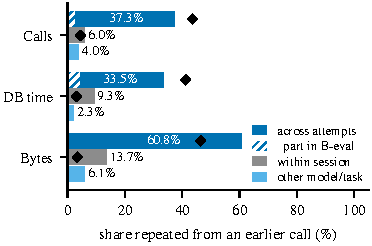
\includegraphics[height=1.62in]{figures/fig1a_scope}}\hfill
  \subcaptionbox{Reuse grows with $N$ (potential tier)\label{fig:ncurve}}{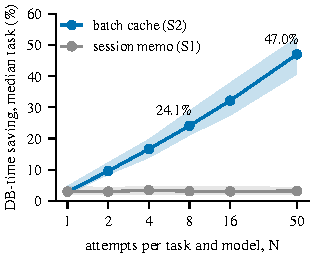
\includegraphics[height=1.62in]{figures/fig1b_ncurve}}\hfill
  \subcaptionbox{What each admission tier admits\label{fig:tiers}}{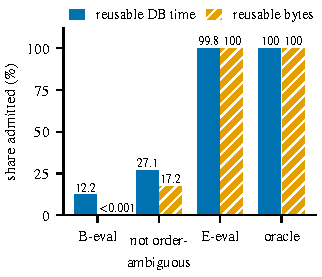
\includegraphics[height=1.62in]{figures/fig1c_tiers}}
  \caption{Where the database work of repeated agent runs repeats, and how much of it each admission tier can reuse
  on DAB. (a) Shares of calls, isolated DB-execution time and payload
  bytes among the 70,173 oracle-admitted calls, by the scope of the earlier exact repeat. The scopes are another
  attempt of the same task and model, the same session, and another model's or task's runs. Shares are pooled over 200
  random attempt orders. Diamonds mark the median task, and hatching marks the part in the B-eval subset. (b)
  Median-task saving of isolated DB-execution time in an unbounded, oracle-gated simulation with 200 resamples. S1 is
  a per-session cache, and S2 is a cache shared by a batch of $N$ attempts of one model on one task. Bands show the
  task-bootstrap 95\% CI, and $N=50$ uses the 268 of 270 task--model cells with 50 runs. (c) Share of the
  cross-attempt reusable DB time and bytes in the B-eval (certified), E-eval (assumption-based) and oracle (potential)
  subsets. The bar ``not order-ambiguous'' covers all calls except the successful ones with at least two distinct rows
  and no top-level \texttt{ORDER BY}. It is a conservative upper bound for any rule that guarantees serialized bytes across query plans in engine row order.}
  \label{fig:teaser}
  \Description{Three panels. Left: horizontal bars showing that repeats across attempts carry 37.3, 33.5 and 60.8 percent of calls, DB time and bytes, against 6.0, 9.3 and 13.7 percent within a session. Middle: lines showing the batch cache saving rising from 3 to 47 percent of DB time as attempts grow from 1 to 50 while the session cache stays near 3 percent. Right: bars showing the B-eval subset holds 12.2 percent of reusable DB time and almost no bytes, the calls that are not order-ambiguous 27.1 percent of the time and 17.2 percent of the bytes, while the E-eval subset and the oracle admit nearly all.}
\end{figure*}

% Table -- the 12 datasets (full width, Section 3)
\begin{table*}[tbp]
  \caption{The 12 DAB datasets of the workload. Columns give the engines (S: SQLite, D: DuckDB, P: PostgreSQL, M:
  MongoDB), the tasks, and the size on disk of the database files and dumps as shipped. They also give the
  \texttt{query\_db} calls, the distinct (database, query) pairs, and the share of successfully replayed calls whose
  result spills to a file. Isolated DB-execution time and payload bytes are summed over all calls. The last columns
  give the median over the dataset's tasks of the DB-time share repeated from other attempts and within the session
  (potential tier).}
  \label{tab:datasets}
  \small
  \begin{tabular}{@{}llrrrrrrrrr@{}}
\toprule
 & & & Data & & Distinct & Spilled & DB time & Bytes & \multicolumn{2}{c}{Task-median repeat \%} \\ \cmidrule(l){10-11}
Dataset & Engines & Tasks & (MB) & Calls & pairs & \% & (s) & (GB) & other attempts & session \\
\midrule
agnews & S, M & 4 & 40.6 & 4,240 & 1,360 & 32.8 & 196 & 11.07 & 41.8 & 2.3 \\
bookreview & S, P & 3 & 1.7 & 3,060 & 1,093 & 49.6 & 5 & 0.11 & 51.8 & 4.3 \\
crmarenapro & S, D, P & 13 & 32.8 & 16,879 & 10,412 & 11.7 & 73 & 0.39 & 35.5 & 1.8 \\
DEPS\_DEV\_V1 & S, D & 2 & 549.9 & 3,125 & 1,281 & 57.1 & 1,874 & 76.06 & 22.3 & 6.9 \\
GITHUB\_REPOS & S, D & 4 & 928.5 & 6,061 & 3,159 & 35.8 & 7,261 & 222.55 & 54.4 & 9.8 \\
googlelocal & S, P & 4 & 0.6 & 3,779 & 1,482 & 16.0 & 5 & 0.03 & 53.9 & 5.0 \\
music\_brainz\_20k & S, D & 3 & 3.1 & 2,451 & 1,071 & 23.2 & 32 & 1.67 & 50.0 & 0.8 \\
PANCANCER\_ATLAS & D, P & 3 & 301.4 & 6,716 & 4,045 & 43.4 & 211 & 1.05 & 37.9 & 3.6 \\
PATENTS & S, P & 3 & 5,556.3 & 4,263 & 2,322 & 63.0 & 23,398 & 225.08 & 36.1 & 7.1 \\
stockindex & S, D & 3 & 4.5 & 2,663 & 1,214 & 25.8 & 64 & 2.70 & 30.7 & 0.6 \\
stockmarket & S, D & 5 & 965.7 & 14,481 & 10,767 & 14.6 & 5,398 & 0.11 & 14.4 & 1.5 \\
yelp & D, M & 7 & 3.7 & 8,495 & 3,410 & 17.2 & 36 & 0.14 & 52.4 & 7.9 \\
\midrule
All &  & 54 & 8,388.9 & 76,213 & 41,616 & 25.9 & 38,553 & 540.96 & 41.2 & 3.2 \\
\bottomrule
\end{tabular}

\end{table*}

% Table -- workload, replay coverage and fidelity by engine (column width, Section 3)
\begin{table}[htbp]
  \caption{Replay coverage and fidelity by engine. Columns give the distinct (database, query) pairs and the share of calls
  whose replay succeeded. They also give the share of successful calls whose replayed result is byte-identical to
  the recorded observation. Byte mismatches differ only in row order or otherwise, and load-time object identifiers
  explain 1,299 of the 1,757 MongoDB mismatches. For spilled results, fidelity compares the 10,000-character preview that the trace keeps.
  The six pairs whose database is not in the task's configuration were not replayed.}
  \label{tab:workload}
  \small\setlength{\tabcolsep}{2.6pt}
  \begin{tabular}{@{}lrrrrrr@{}}
\toprule
 & & Distinct & Replay & Byte- & \multicolumn{2}{c}{Mismatches} \\ \cmidrule(l){6-7}
Engine & Calls & pairs & ok \% & identical \% & order & other \\
\midrule
DuckDB & 29,145 & 18,569 & 94.0 & 91.7 & 1,743 & 520 \\
MongoDB & 8,508 & 3,292 & 96.4 & 78.5 & 0 & 1,757 \\
PostgreSQL & 19,033 & 11,712 & 88.4 & 94.3 & 547 & 406 \\
SQLite & 19,455 & 8,037 & 98.5 & 99.9 & 0 & 4 \\
\midrule
All & 76,213 & 41,616 & 93.9 & 93.0 & 2,290 & 2,687 \\
\bottomrule
\end{tabular}

\end{table}

% Table -- admission tiers (column width, Section 3)
\begin{table}[htbp]
  \caption{Admission tiers and the calls each admits (of 76,213). ``Online'' means decidable before the call executes.
  The B-eval and E-eval subsets keep the calls of each static rule whose replay was byte-identical to the recorded
  observation and stable over three replays. They are post-hoc restrictions on which we measure designs.}
  \label{tab:tiers}
  \small\setlength{\tabcolsep}{3pt}
  \begin{tabular}{@{}L{1.55cm}L{3.75cm}cr@{}}
\toprule
Tier & Admission rule & Online & Calls \\
\midrule
Certified & Contract B: conditional static byte-stability certificate & yes & 5,697 \\
 & \quad B-eval subset (post hoc) & no & 5,695 \\
Assumption-based & static Contract E, byte stability from a pinned runtime & yes & 74,894 \\
 & \quad E-eval subset (post hoc) & no & 66,263 \\
Potential & oracle: replay equivalent to the recorded observation & no & 70,173 \\
\bottomrule
\end{tabular}

\end{table}

% Table -- Contract B in full (column width, Section 3)
\begin{table}[htbp]
  \caption{Summary of Contract B's construct whitelist. Admission also applies the schema-binding, type-family,
  argument-form, alias and potentially-raising-expression checks of the artifact. $c$: a stored column that satisfies P2.}
  \label{tab:contractb}
  \footnotesize\setlength{\tabcolsep}{3pt}
  \begin{tabular}{@{}L{1.25cm}L{6.7cm}@{}}
  \toprule
  Statement & one \texttt{SELECT} block; no \texttt{WITH}, subquery, set operation, window, \texttt{DISTINCT ON},
  \texttt{VALUES} or table function \\
  \texttt{FROM} & base tables of the audited schema, joined by \texttt{JOIN}\,\ldots\,\texttt{ON} or a comma; no
  \texttt{USING}, \texttt{NATURAL} or \texttt{LATERAL} \\
  Names & each column binds to exactly one stored column of the tables in scope (ASCII names, the engine's case
  rule); an output alias does not shadow another column \\
  Row\newline expression & in \texttt{WHERE}, \texttt{ON} and the argument of \texttt{COUNT}: columns; literals without
  clock words; comparisons; \texttt{AND}, \texttt{OR}, \texttt{NOT}; \texttt{IS NULL}; \texttt{IN} over a list;
  \texttt{BETWEEN}; \texttt{LIKE} with a literal pattern; searched \texttt{CASE}; \texttt{COALESCE};
  \texttt{LOWER}, \texttt{UPPER}, \texttt{LENGTH}, \texttt{TRIM}, \texttt{REPLACE}. SQLite also: arithmetic,
  \texttt{ROUND}, \texttt{SUBSTR}, casts. DuckDB also: \texttt{SUBSTR}, \texttt{TRY\_CAST}, and arithmetic,
  \texttt{ABS} and \texttt{ROUND} over floating-point columns; a string meets only strings in a comparison \\
  One row & no \texttt{GROUP BY}, \texttt{HAVING}, \texttt{ORDER BY}, \texttt{OFFSET} or \texttt{DISTINCT}; each
  output built from \texttt{COUNT}, \texttt{MIN}($c$), \texttt{MAX}($c$), literals, arithmetic and the functions above \\
  Ordered & no aggregate; each output is a column $c$; \texttt{ORDER BY} names every output \\
  Grouped & \texttt{GROUP BY} columns $c$; each output is a grouping column or one \texttt{COUNT},
  \texttt{MIN}($c$) or \texttt{MAX}($c$); \texttt{HAVING} over such aggregates; \texttt{ORDER BY} names every
  grouping column, or every output \\
  Limits & \texttt{LIMIT} (at least one row) and \texttt{OFFSET} take integer literals; plain \texttt{DISTINCT}
  needs an \texttt{ORDER BY} over every output \\
  \bottomrule
  \end{tabular}
\end{table}

% Fig. 2 -- locality per task and under different conditions (figure*, Section 4)
\begin{figure*}[tbp]
  \centering
  \subcaptionbox{Per task: session share against cross-attempt share\label{fig:pertask}}{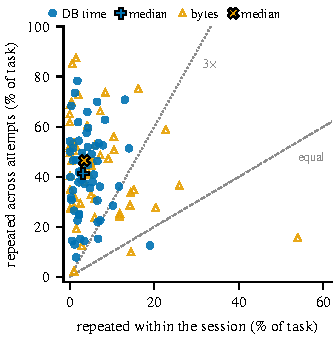
\includegraphics[height=2.05in]{figures/fig2a_pertask}}\hfill
  \subcaptionbox{Pooled share of isolated DB-execution time under different conditions\label{fig:conditions}}{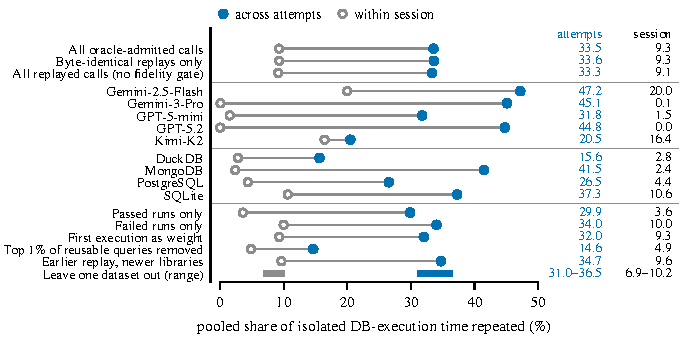
\includegraphics[height=2.05in]{figures/fig2b_conditions}}
  \caption{Locality per task and under different conditions. (a) One point per task and weight for the 54 tasks, on the oracle-admitted calls. Circles show isolated
  DB-execution time and triangles payload bytes. The axes give the share repeated within the session ($x$) and
  across attempts of the same task and model ($y$). The dashed line is $y=x$, the dotted line is
  $y=3x$, and large markers are task medians. (b) Pooled DB-time shares on the 70,173 oracle-admitted calls, a named
  subset, or another population. Byte-identical replays cover 66,556 calls, all replayed calls 76,141, and the earlier
  replay its 62,419 byte-identical calls. Shares are means over 200 random attempt orders, with 20 orders for the two
  gate variants and 50 for the top-1\% removal.}
  \label{fig:locality}
  \Description{Two panels. Left: a scatter plot with two points per task, one for DB time and one for bytes. Nearly all lie above the equal-share line and most above the three-times line. Right: one row per condition. The cross-attempt estimate lies to the right of the within-session estimate in every row, with the leave-one-dataset-out row shown as ranges.}
\end{figure*}

% Table 4 -- cross-harness (column width)
\begin{table}[htbp]
  \caption{Exact-call repetition in four public leaderboard harnesses on DAB's tasks and in the first five runs of the
  released DAB traces. The analysis is at trace level, without replay, on the exact database and query text. Qwen3.8
  denotes Qwen3.8-Flash-Next, and DeepSeek-v4.1 denotes DeepSeek-v4.1-flash. Session and other-attempt columns are
  pooled call shares averaged over 50 random attempt orders. $N{=}5$ is the median share of calls that repeat an
  earlier call among five attempts (50 resamples), over the listed number of tasks with five available runs.}
  \label{tab:xharness}
  \footnotesize\setlength{\tabcolsep}{2.5pt}
  \begin{tabular}{@{}lrrrrr@{}}
\toprule
Harness / model & Runs & Calls & \% session & \% other att. & $N{=}5$ \% (tasks) \\
\midrule
Phoenix-CLI / Opus 5 & 270 & 2,937 & 1.7 & 13.4 & 15.5 (54) \\
DAB scaffold / Qwen3.8 & 270 & 3,294 & 0.1 & 15.9 & 17.9 (54) \\
Scout / GLM-5.2 & 249 & 1,490 & 0.3 & 5.7 & 7.8 (37) \\
Stela / DeepSeek-v4.1 & 264 & 3,306 & 0.2 & 5.0 & 4.9 (48) \\
\midrule
DAB / Gemini-2.5-Flash & 269 & 958 & 18.7 & 14.7 & 30.0 (53) \\
DAB / Gemini-3-Pro & 270 & 1,708 & 0.1 & 23.2 & 24.6 (54) \\
DAB / GPT-5-mini & 270 & 1,388 & 0.5 & 8.6 & 11.2 (54) \\
DAB / GPT-5.2 & 270 & 1,093 & 0.1 & 13.5 & 13.2 (54) \\
DAB / Kimi-K2 & 266 & 2,287 & 11.6 & 8.3 & 13.3 (51) \\
\bottomrule
\end{tabular}

\end{table}

% Table 1 -- funnel (column width)
\begin{table}[htbp]
  \caption{Admission funnel over all 76,213 database calls: pooled shares of calls, isolated DB-execution time (a
  timeout counts at the 120\,s cap) and payload bytes. Gates are cumulative. The last two rows are the post-hoc E-eval
  (assumption-based) and B-eval (certified) subsets. They hold the calls of the static E and B rules whose replay is
  byte-identical to the recorded observation and stable across three replays. The oracle (potential) admits every call
  whose replay is equivalent to the recorded observation.}
  \label{tab:funnel}
  \small\setlength{\tabcolsep}{3pt}
  \begin{tabular}{@{}L{3.15cm}rrrr@{}}
\toprule
Gate (cumulative) & Calls & \% calls & \% DB time & \% bytes \\
\midrule
Successful replay & 71,582 & 93.9 & 94.7 & 100.0 \\
Equivalent to recorded observation (oracle) & 70,173 & 92.1 & 94.2 & 98.8 \\
Byte-identical, stable in 3 replays & 66,556 & 87.3 & 93.9 & 98.8 \\
E-eval subset (static E, post hoc) & 66,263 & 86.9 & 93.6 & 98.7 \\
B-eval subset (static B, post hoc) & 5,695 & 7.5 & 9.4 & 0.023 \\
\bottomrule
\end{tabular}

\end{table}

% Fig. 3 -- admission per engine and the verdicts of the static Contract B rule (column width, Section 5)
\begin{figure}[htbp]
  \centering
  \subcaptionbox{The funnel of Table~\ref{tab:funnel} per engine\label{fig:funnelengine}}{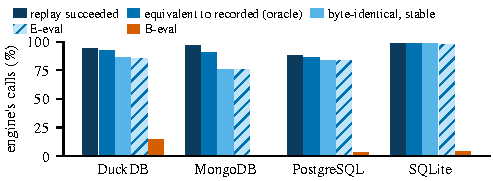
\includegraphics[width=\columnwidth]{figures/fig3a_funnel_engine}}
  \subcaptionbox{Verdicts of the static Contract B rule\label{fig:verdicts}}{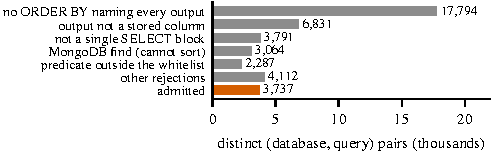
\includegraphics[width=\columnwidth]{figures/fig3b_b_verdicts}}
  \caption{Admission by engine and by rule. (a) Share of each engine's calls that passes each cumulative gate of Table~\ref{tab:funnel}. It covers the 76,141 calls with a replay outcome, and Table~\ref{tab:workload} gives the totals.
  MongoDB's B-eval subset, two calls, is too small to see. (b) Verdict of the static Contract B rule on each of the 41,616 distinct (database, query) pairs. Bars show rejection reasons and the admitted pairs.}
  \label{fig:certify}
  \Description{Two panels. Top: grouped bars per engine showing that most calls of every engine pass the replay, equivalence, byte-identity and E-eval gates, while the B-eval subset is a small share. Bottom: horizontal bars of the number of distinct (database, query) pairs per verdict of the static Contract B rule. The longest bar is the rejection for lacking an ORDER BY that names every output.}
\end{figure}

% Fig. 4 -- ownership (column width, Section 6)
\begin{figure}[htbp]
  \centering
  \subcaptionbox{Tool-boundary result ownership and the lifetime of a shared object\label{fig:designs}}{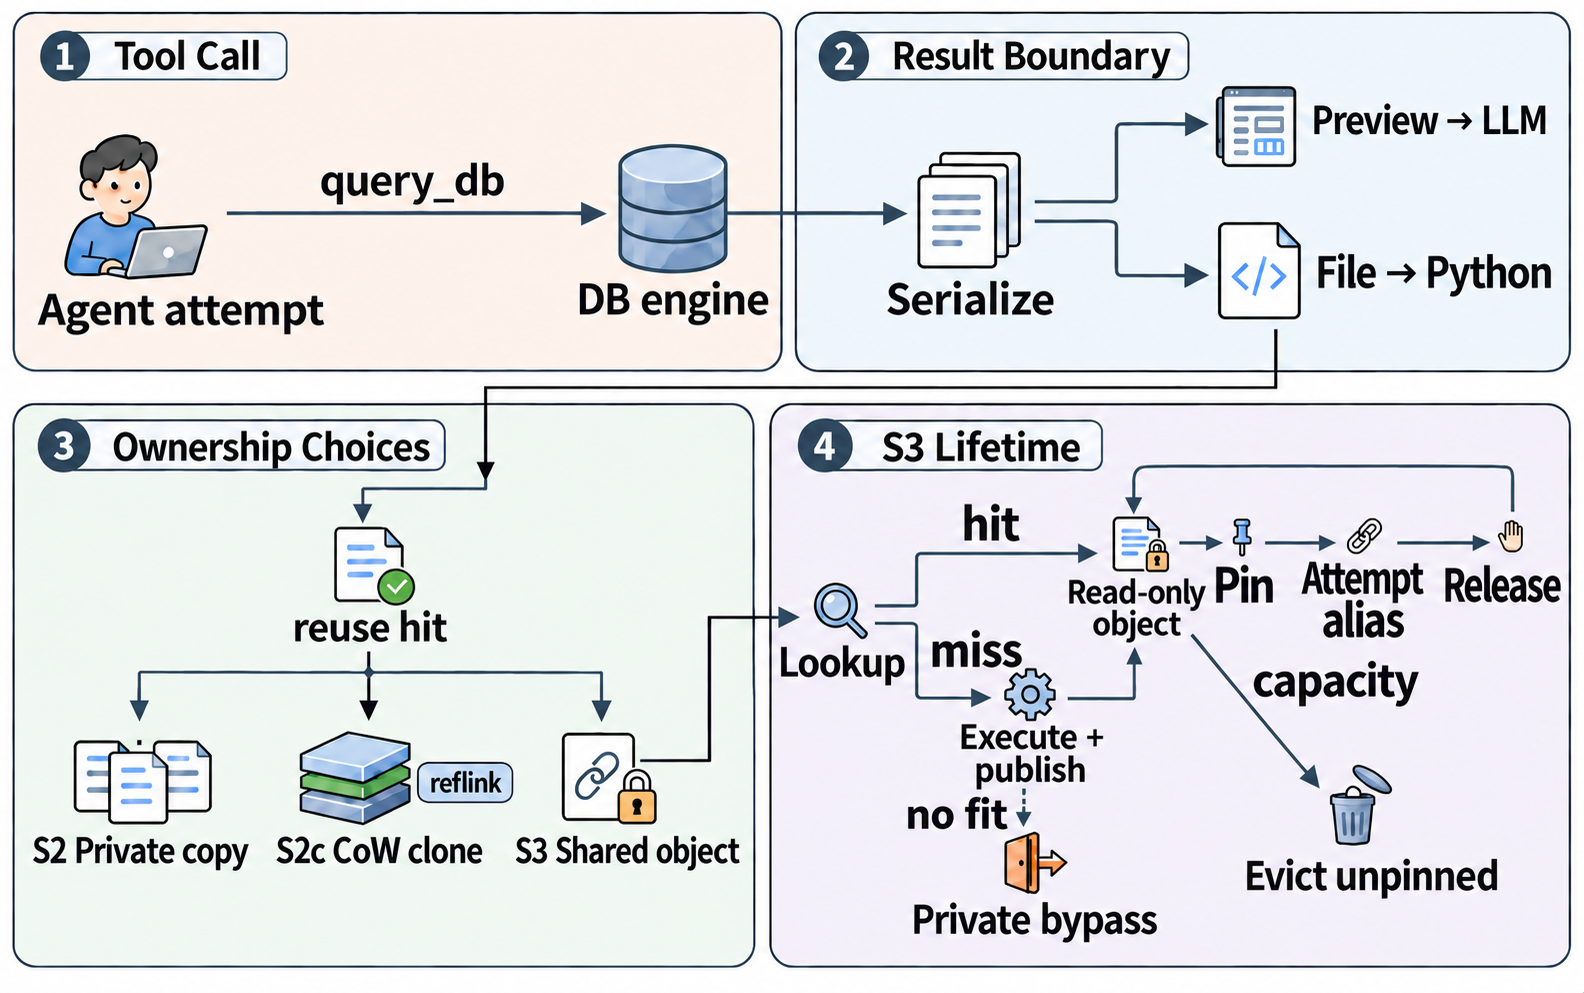
\includegraphics[width=\columnwidth]{figures/fig4a_ownership}}\\[3pt]
  \subcaptionbox{Footprint vs.\ $N$\label{fig:footN}}{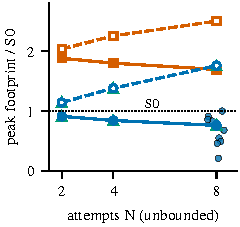
\includegraphics[height=1.45in]{figures/fig4b_footprint_N}}\hfill
  \subcaptionbox{Footprint vs.\ budget\label{fig:footB}}{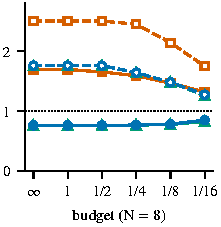
\includegraphics[height=1.45in]{figures/fig4c_footprint_budget}}\\[1pt]
  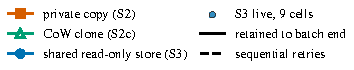
\includegraphics{figures/fig4_legend}
  \caption{Result ownership decides storage cost. (a) A \texttt{query\_db} result is serialized into an LLM preview and a file for Python. Only the file takes part in ownership. On a hit, S2 provides a private copy and S2c a reflink clone. S3 aliases one shared read-only object. SD is omitted because it changes execution but retains attempt-private serialization and files. Section~\ref{sec:designs} describes the lifetime of an S3 object. (b, c) Simulated peak footprint relative to no sharing (S0) on the assumption-based E-eval subset. Values are medians over the 52 tasks with nonzero S0 footprint (50 resamples). Panel (b) uses an unbounded budget and panel (c) uses $N=8$.
  Solid lines retain outputs to batch end, and dashed lines are sequential retries. Dots in (b) are live S3/S0 on the
  9 calibration cells with admitted spilled bytes ($N=8$, unbounded budget, median of 5 resamples, jittered). The
  simulator reproduces each cell.}
  \label{fig:ownership}
  \Description{Top: a four-region diagram. Region 1 shows an agent attempt calling query_db on a database engine. Region 2 shows the result serialized into a preview for the LLM and a file for Python. Region 3 shows three ownership choices on a reuse hit: a private copy, a copy-on-write clone, and a shared object. Region 4 shows the lifetime of a shared object: lookup, hit or miss with execute and publish, pin, attempt alias, release, eviction of unpinned objects under capacity pressure, and a private bypass when a result does not fit. Bottom: two line plots of peak footprint relative to no sharing. Private copies stay above 1, the shared store and clones stay near 0.76 to 0.91 when outputs are retained and between 1.14 and 1.76 for sequential retries.}
\end{figure}

% Table 2 -- designs (full width)
\begin{table*}[tbp]
  \caption{Reuse designs at $N=8$ with an unbounded budget on the assumption-based E-eval subset (simulation, 50
  resamples). DB-execution saving relative to S0 is the median over 54 tasks. Bytes written and peak footprint
  relative to S0 are medians over the 52 tasks with nonzero S0 writes, under the retained and sequential lifetimes of
  Section~\ref{sec:designs}. Both are exact accounting. Modeled tool-time saving is the simulator's estimate (median
  over 54 tasks), with a per-run error of 43.9\% on this subset. The live calibration
  compares S2, S2c and S3, and SD's tool time is modeled only. Measured primitives are the live copy rate per byte
  (258 copies) and the clone (482) and alias (282) times.}
  \label{tab:designs}
  \small
  \begin{tabular}{@{}lrrrrlr@{}}
\toprule
 & DB-time & Written & \multicolumn{2}{c}{Footprint / S0} & Measured & Modeled tool-time \\
\cmidrule(lr){4-5}
Design & saving \% & / S0 & retained & sequential & primitive & saving \% \\
\midrule
Isolated (S0) & 0.0 & 1.00 & 1.00 & 1.00 & --- & 0.0 \\
Session memo (S1) & 3.4 & 0.98 & 0.98 & 0.96 & --- & 3.4 \\
Execution-only cache model (SD) & 24.5 & 1.00 & 1.00 & 1.00 & --- & 11.8 \\
Private copy (S2) & 24.5 & 1.70 & 1.70 & 2.50 & copy 0.46 ns/B & 24.9 \\
CoW clone (S2c) & 24.5 & 0.76 & 0.76 & 1.76 & clone 0.29 ms & 24.8 \\
Shared read-only store (S3) & 24.5 & 0.76 & 0.76 & 1.76 & alias 12.6\,\textmu s & 25.0 \\
\bottomrule
\end{tabular}

\end{table*}

% Table 3 -- correctness (a) and concurrency (b) (full width, stacked)
\begin{table*}[tbp]
  \caption{Observations under reuse on the assumption-based E-eval subset, $N=8$. (a) Live trace replay of S3 against
  S0 on identical attempt orders. The passes cover all 270 task--model cells (one resample, unbounded budget) and a
  one-worker rerun of the 15 PATENTS cells on the same attempt orders. They also cover the 12 calibration cells
  (budgets $\infty$ and 1/4, two resamples) and a CoW pass on 8 of them. ``Hits $\neq$ S0'' counts cached hits whose
  observation differs from S0. ``Value mismatches'' counts hits where S0 and S3 both returned a result and the
  results differ. The 2 differing hits of the all-cell pass are PATENTS calls whose S0 execution failed under load
  while S3 returned a result. ``Consumers'' counts recorded agent Python code re-run with identical successes,
  identical failures, and differing output. The 2 differing consumers in the CoW pass are S0 timeouts at the 120\,s
  cap. (b) The 8 attempts of each calibration cell as concurrent threads against one S3 store (2 resamples, 757 calls
  per configuration), compared with a serial S0 run.}
  \label{tab:e2e}
  \small
  \subcaptionbox{Live trace replay: S3 against S0\label{tab:e2e-a}}{\begin{tabular}{@{}lrrrrrcc@{}}
\toprule
Pass (S3 vs.\ S0) & Cells & Calls & Hits & Hits $\neq$ S0 & Value mismatches & Consumers same ok\,/\,fail\,/\,diff & Probes refused\,/\,total \\
\midrule
All cells, $\infty$ & 270 & 11,309 & 2,443 & 2 & 0 & 3,381\,/\,1,274\,/\,0 & 630\,/\,630 \\
PATENTS rerun, $\infty$ & 15 & 632 & 159 & 0 & 0 & 289\,/\,102\,/\,0 & 45\,/\,45 \\
Calibration, $\infty$, 1/4 & 12 & 1,394 & 310 & 0 & 0 & 742\,/\,76\,/\,0 & 114\,/\,114 \\
Calibration, CoW pass & 8 & 844 & 162 & 0 & 0 & 434\,/\,46\,/\,2 & 72\,/\,72 \\
\bottomrule
\end{tabular}
}\\[4pt]
  \subcaptionbox{Concurrent attempts against one S3 store\label{tab:e2e-b}}{\begin{tabular}{@{}llrrrrr@{}}
\toprule
Budget & Policy & Mismatches & Executions & Duplicates & Wait (s) & Dangling aliases \\
\midrule
$\infty$ & optimistic & 0 & 663 & 107 & 0 & 0 \\
$\infty$ & single-flight & 0 & 556 & 0 & 59 & 0 \\
$\infty$ & optimistic, unpinned & 0 & 664 & 108 & 0 & 0 \\
1/16 & optimistic & 0 & 675 & 103 & 0 & 0 \\
1/16 & single-flight & 0 & 567 & 0 & 86 & 0 \\
1/16 & optimistic, unpinned & 0 & 681 & 106 & 0 & 21 \\
\bottomrule
\end{tabular}
}
\end{table*}

% Table -- pre-specified analyses (full width, Section 7)
\begin{table*}[tbp]
  \caption{Pre-specified analyses and thresholds, fixed in the experiment plan after the pilot and before the full
  replay, and outcomes. Contract B evolved after the plan (Section~\ref{sec:threats}). The outcomes that depend on it
  are given for the rule as planned and for the final rule.}
  \label{tab:prereg}
  \small
  \begin{tabular}{@{}L{3.3cm}L{6.1cm}L{6.7cm}@{}}
\toprule
Analysis & Threshold & Outcome \\
\midrule
B0 replay fidelity & replayed result byte-identical to the recorded observation for $\geq$90\% of the successful calls of every engine & met for DuckDB, PostgreSQL and SQLite (91.7\%, 94.3\%, 99.9\%); MongoDB 78.5\%, and 94.4\% equivalent after the normalization of Section~\ref{sec:method} \\
B1 cross-attempt dominance & other attempts $\geq 3\times$ session in time and bytes, pooled and for the median task, on byte-identical replays of the engines that meet B0 & met on that population (three engines): 3.6$\times$ (time), 4.4$\times$ (bytes) pooled; 14.9$\times$, 12.6$\times$ for the median task. On all oracle-admitted calls (Section~\ref{sec:locality}): 3.6$\times$, 4.4$\times$; 13.0$\times$, 13.4$\times$ \\
B2 practical savings & under S2, the median task saves $\geq$20\% of DB time or $\geq$30\% of bytes at $N=4$ & not met at $N=4$ on the oracle-admitted calls with an unbounded budget (16.6\%, 15.9\%); 24.1\% of DB time at $N=8$ \\
B3 ownership & on the calls that Contract B admits, at $N=2$--8: S3 below S2 in median-task bytes written and peak footprint, tool time within 5\%, same direction in every engine & not met on Contract B, which admits a spilled result in only 11 tasks as planned and 8 under the final rule, with a median S3 write saving of 0\% and 0\%; met on E-eval (exploratory, unbounded budget): S3/S2 writes 0.448--0.489, footprint 0.448--0.696 under both lifetimes, tool time 0.998--0.999; in every engine, writes at most 0.63 and tool time at most 1.03 (footprint was not computed per engine) \\
B4 simulator validity and consumer test & on 12 calibration cells at $N=8$ with an unbounded and a 1/4 budget: simulated tool time within 10\%, bytes within 1\%; consumer outputs identical in $\geq$99\% of cases; writes to shared objects refused & bytes and footprint met (max error 0\%); tool time 8.6\% under B as planned (met), 30.6\% under the final B and 43.9\% on E-eval (not met); consumer test, planned on inputs that Contract B admits and run on E-eval inputs, on 238 recorded Python calls: 238 outputs identical under S2 and S3 with the hash seed fixed (233 with random seeds), 36 of 36 write probes refused by a read-only mount (met) \\
B5 heterogeneity & B1 holds in $\geq 10$ of 12 leave-one-dataset-out folds and for every model & on the B1 population, met in 12 of 12 folds (smallest ratio 3.4$\times$ in time, 4.0$\times$ in bytes) and for 3 of 5 models \\
\bottomrule
\end{tabular}

\end{table*}
